\section{Непрерывные функции. Предел функции в точке.}

Пусть $E \subset \mathds{R}, \ a,b \in \overline{\mathds{R}}, f: E \longrightarrow \mathds{R}$
\begin{definition}{\textit{Коши.}}
    Точка $b$ называется \underline{пределом функции} $f$ в точке $a$, если $a$ -- предельная точка множества $E$ и 
    \[\forall \epsilon > 0 \ \exists \delta > 0 \ \forall x \in E \ (x \in \overset{o}{B_{\delta}}(a) \Rightarrow f(x) \in \overset{}{B_{\epsilon}}(b))\]
    Пишут: $\lim_{x \rightarrow a} f(x) =  b$ или $f(x) \rightarrow b$ при $x \rightarrow a$.
\end{definition}

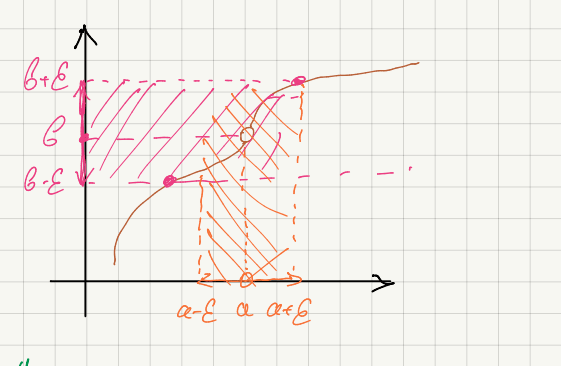
\includegraphics[width=0.6\textwidth]{ex1.png}

\begin{note}
    Если $E =\mathds{N}$, $a = +\infty$, то получим $\lim_{} \{a_{n}\} \ (n_{0} = [\frac{1}{\delta}] + 1)$.
\end{note}

\begin{definition}{\textit{Гейне.}}
    Точка $b$ называется \underline{пределом функции} $f$ в точке $a$, если $a$ -- предельная точка $E$ и выпонено следующее:
    \[\forall\{x_{n}\} \subset E \setminus \{a\} \ (\{x_{n}\} \rightarrow a \Rightarrow f(x_{n}) \rightarrow b )\]
    Пишут: $\lim_{x \rightarrow a} f(x) =  b$ или $f(x) \rightarrow b$ при $x \rightarrow a$.
\end{definition}

\begin{note}
    Так как $a$ -- предельная точка множества $E$, то $\forall \delta > 0 \ \overset{o}{B_{\epsilon}}(a) \cap E \neq \emptyset$ и $\exists \{x_{n}\} \subset E \setminus \{a\}$: $x_{n} \rightarrow a$.
\end{note}

\begin{theorem}
    Определения пределов по Коши и по Гейне равносильны.
\end{theorem}

\begin{proof}
    Пусть $f: E \longrightarrow R$, $a$ -- предельная точка множества $E$.
    \\
    $\Rightarrow$ Пусть $b = \lim_{x \rightarrow a} f(x)$ по Коши.
    Рассмотрим произвольную $\{x_{n}\} \subset E \setminus \{a\}$, $x_{n} \rightarrow a$. Докажем, что $f(x_{n}) \rightarrow b$.
    \\
    Зафиксируем $\epsilon > 0$. По определению предела $\exists \delta > 0 \ \forall x \in E \ (x \in \overset{o}{B_{\delta}}(a) \Rightarrow f(x) \in \overset{}{B_{\epsilon}}(b))$. Т.к. $x_{n} \rightarrow a$, то $\exists N \in \mathds{N} \ \forall n \geq N \ (x_{n} \in \overset{}{B_{\delta}}(a))$. По условию $x_{n} \in E \setminus \{a\}$ и, значит, $\forall n \geq N \ (x_{n} \in \overset{o}{B_{\delta}}(a) \cap E)$. Тогда $\forall n \geq N: f(x_{n}) \in \overset{}{B_{\epsilon}}(b) \Rightarrow f(x_{n}) \rightarrow b$. Определение предела по Гейне выполняется. 
    \\
    $\Leftarrow$ Пусть $b$ -- предел $f$ в точке $a$ по Гейне. Покажем, что $b$ -- предел функции по Коши. Пусть так, и предположим, что $b$ не является пределом $f$ в точке $a$ по Коши. Тогда 
    \[\exists \epsilon > 0 \ \forall \delta \ \exists x \in E (x \in \overset{o}{B_{\delta}}(a) \text{ и } f(x) \notin \overset{}{B_{\epsilon}}(b))\]
    Положим $\delta = \frac{1}{n}$, $n \in \mathds{N}$ и соответствующее значение x обозначим $x_{n}$. По построению $\{x_{n}\} \subset E \setminus \{a\}$ и $x_{n} \rightarrow a$ (т.к. $x_{n} \in \overset{}{B_{\frac{1}{n}}}(a)$). По определению предела по Гейне $f(x_{n}) \rightarrow b$, значит $\exists N \in \mathds{N} (f(x_{n}) \in \overset{}{B_{\epsilon}}(b))$. Противоречие по построению (все $f(x_{n}) \notin \overset{}{B_{\epsilon}}(b)$).
\end{proof}

\begin{note}
    Распишем определение предела по Коши в частном случае, когда $a$, $b$ -- числа, на языке неравенств.
    \\
    \[b = \lim_{x \rightarrow a} f(x) \lra \text{$a$ -- предельная точка $f$}\]
    \[\forall \epsilon > 0 \ \exists \delta > 0 \ \forall x \in E (0 < |x - a| < \delta \Rightarrow |f(x_{n}) - b| < \epsilon)\]
\end{note}

\subsection{Свойства предела функции.}
Пусть $f,g,h: E \longrightarrow \mathds{R}$, $a$ -- предельная точка множества $E$.

\begin{definition}
    $f: X \longrightarrow Y$, $A \subset X$. \underline{Сужением} $f$ на множестве $A$ называется
    \[f|_{A}: A \longrightarrow Y, (f|_{A})(x) = f(x) \ \forall x \in A\]
\end{definition}

\begin{enumerate}
    \item (о единственности) Если $\lim_{x \rightarrow a} f(x) = b$ и $\lim_{x \rightarrow a} f(x) = c$, то $b = c$
    \begin{proof}
        Рассмотрим произвольную $\{x_{n}\} \subset E \setminus \{a\}$, $x_{n} \rightarrow a$. По определению Гейне:
        \[f(x_{n}) \rightarrow b \text{ и } f(x_{n}) \rightarrow c\]
        В силу единственности предела последовательности $b = c$.
    \end{proof}
    \item (о пределе по подмножеству) Если $\lim_{x \rightarrow a} f(x) = b$ и $a$ -- предельная точка множества $D \subset E$, то $\lim_{x \rightarrow a} f|_{D}(x) = b$.
    \begin{proof}
        Рассмотрим $\{x_{n}\} \subset D \setminus \{a\}$, $x_{n} \rightarrow a$. Тогда
        \[f|_{D}(x_{n}) = f(x_{n}) \rightarrow b\]
        По определению Гейне, $b = \lim_{x \rightarrow a} f|_{D}(x)$.
    \end{proof}
    \item (о зажатой функции) Пусть $\exists \sigma > 0 \ \forall x \in \overset{o}{B_{\delta}} (a) \cap E \ (f(x) \leq h(x) \leq g(x))$. Пусть $\lim_{x \rightarrow a} f(x) = b$, $\lim_{x \rightarrow a} g(x) = b$. Тогда $\exists \lim_{x \rightarrow a} h(x) = b$.
    \begin{proof}
        Рассмотрим $x_{n} \subset E \setminus \{a\}$, $x_{n} \rightarrow a$. Тогда $\exists n_{0} \ \forall n \geq n_{0} (x_{n} \in \overset{o}{B_{\delta}}(a) \cap E)$ и, значит, $f(x_{n}) \leq h(x_{n}) \leq g(x_{n})$. По условию $f(x_{n}) \rightarrow b$, $g(x_{n}) \rightarrow b$. Тогда, по свойству предела последовательности, $h(x_{n}) \rightarrow b \Rightarrow b = \lim_{x \rightarrow a} h(x)$.
    \end{proof}
    \item (арифметические опреации с пределами) Пусть $\lim_{x \rightarrow a} f(x) = b$, $\lim_{x \rightarrow a} g(x) = c$. Тогда справедливы следующие утверждения:
    \\
    1. $\lim_{x \rightarrow a} (f(x) \pm g(x)) = b \pm c$.
    \\
    2. $\lim_{x \rightarrow a} (f(x) \cdot g(x)) = b \cdot c$.
    \\
    3. Если $c \neq 0$ и $g(x) \neq 0 \ \forall x \in E$, то $\lim_{x \rightarrow a} (\frac{f(x)}{g(x)}) = \frac{b}{c}$.
    
    Заключение следует понимать так: если существует величина справа, то существует величина слева и они равны.
    \begin{proof}
        Рассмотрим произвольную последовательность $\{x_{n}\} \in E$ с условиями $x_{n} \to a$ и $x_{n} \neq a$. Тогда $f(x_{n}) \to b$ и $g(x_{n}) \to c$. По свойствам предела последовательности $f(x_{n}) \pm g(x_{n}) \to b \pm c$, $f(x_{n}) \cdot g(x_{n}) \to b \cdot c$, $\frac{f(x_{n})}{g(x_{n})} \to \frac{b}{c}$. Осталось воспользоваться определением предела по Гейне.
    \end{proof}
    \item (о локализации) Если $\exists \sigma > 0 \ \forall x \in \overset{o}{B_{\sigma}}(a) \cap E \ (f(x) = g(x))$ и $\lim_{x \rightarrow a} f(x) = b$, то $\exists \lim_{x \rightarrow a} g(x) = b$.
    \begin{proof}
        Если в определении Коши предел $f$ для $\epsilon > 0$ подходит $\delta > 0$, то в поределении Коши предел $g$ подходит $\delta' = min\{\delta, \sigma\}$.
    \end{proof}
    \item (о локализации ограниченности) Если $\exists \lim_{x \rightarrow a} f(x) \in \mathds{R}$, то $\exists C > 0 \ \exists \delta > 0 \ \forall x \in \overset{o}{B_{\delta}}(a) \cap E \ (|f(x)| \leq C)$.
    \begin{proof}
        Пусть $\lim_{x \rightarrow a} f(x) = b$. Тогда $\exists \delta > 0 \ \forall x \in \overset{o}{B_{\delta}}(a) \cap E \ (b - 1 < f(x) < b + 1)$. Положим $c = |b| + 1$. Тогда $|f(x)| < c$.
    \end{proof}
    \item (О пределе композиции.) Пусть $E, D \subset \mathds{R}$ и $f: E \longrightarrow D$ и $g: D \longrightarrow \mathds{R}$, такие что $\lim_{x \rightarrow a} f(x) = b$ и $\lim_{y \rightarrow b} g(y) = c$. Пусть выполнено одно из двух условий: 
    \\
    1) $f(x) \neq b$ в некоторой проколотой окрестности множества $a$ или 
    \\
    2) $g(b) = c$. Тогда $\lim_{x \rightarrow a} g(f(x)) = c = \lim_{y \rightarrow b} g(y)$.
    \begin{proof}
        Зафиксируем $\epsilon > 0$. По определению предела
        \[\exists \sigma > 0 \ \forall y \in \overset{o}{B_{\sigma}}(b) \cap D \ (g(y) \in \overset{}{B_{\epsilon}}(c))\]
        \[\exists \delta > 0 \ \forall y \in \overset{o}{B_{\delta}}(a) \cap E \ (f(x) \in \overset{}{B_{\sigma}}(b))\]
        1) Уменьшая $\delta$, если необходимо, можно считать, что $f(x) \neq b$ на $\overset{o}{B_{\delta}}(a) \cap E$. Тогда $f(x) \in \overset{o}{B_{\sigma}}(b) \cap D$. Поэтому $g(f(x)) \in \overset{}{B_{\epsilon}}(c) \Rightarrow \lim_{x \rightarrow a} g(f(x)) = c$.
        \\
        2) Если $f(x) = b$ для некоторого $x \in \overset{}{B_{\delta}}(a)$, то $g(f(x)) = c \in \overset{}{B_{\epsilon}}(c)$. Поэтому $\forall x \in \overset{}{B_{\delta}}(a) \cap E \ (g(f(x)) \in \overset{}{B_{\epsilon}}(c)) \Rightarrow \lim_{x \rightarrow a} g(f(x)) = c$.
    \end{proof}
\end{enumerate}